\documentclass{article}
\usepackage[utf8]{inputenc}
\usepackage[slovene]{babel}
\usepackage{graphicx}
\usepackage{subfigure}
\usepackage{amsfonts} 
\usepackage{amsmath}
\usepackage{hyperref}
\usepackage{listings}

\newcommand{\program}{Finanča matematika} 
\newcommand{\imeavtorja}{Anja Plesec}
\newcommand{\imementorja}{prof.~dr.~ Sergio Cabello Justo, \\ asist. Gašper Domen Romih}
\newcommand{\naslovdela}{Gradientni spust}
\newcommand{\letnica}{2022}

\begin{document}

\thispagestyle{empty}
\noindent{\large
UNIVERZA V LJUBLJANI\\[1mm]
FAKULTETA ZA MATEMATIKO IN FIZIKO\\[5mm]
\program\ -- 2.~stopnja}
\vfill

\begin{center}{\large
\imeavtorja\\[2mm]
{\bf \naslovdela}\\[10mm]
Končno poročilo pri predmetu Matematika z računalnikom\\[1cm]
Mentor: \imementorja}
\end{center}
\vfill

\noindent{\large
Ljubljana, \letnica}
\pagebreak

\newpage


\section{Uvod}
V projektni nalogi predstavim metodo gradientnega spusta. Na enostaven način bi lahko to metodo opisala takole: stojimo na vrhu hriba in si želimo priti do doline. Ker hriba ne poznamo se odpravimo po poti navzdol, ki je najbolj strma. Na začetku delamo velike korake, ko pa pot postaja bolj položna začnemo delati manjše korake, saj bomo kmalu prispeli na cilj - v dolino. Na vsakem koraku je naslednji korak odvisen od lokacije, kjer se nahajamo in strmine hriba. Na isti način deluje tudi metoda gradientnega spusta, ki jo bom predstavila skozi nalogo. Projekt sem izdelala v programu Matlab, kjer sem si naprej pogledala uporabo gradientnega spusta v primeru linearne regresije, nato pa na funkcijah ene in več spremenljivk.

\section{Teoretična izhodišča}
Gradientni spust je iterativna metoda za iskanje lokalnega minimuma funkcije, ki se lahko uporablja na različnih področjih. Ideja metode je, da najdemo minimum funkcije: 
\[\min_{x \in \mathbb{R}^n} f(x),\]
kjer predpostavimo, da je funkcija f konveksna in diferenciabilna v vsaki točki. Naj obstaja optimalna točka $y^*$ in predpostavimo, da obstaja tak $x^*$, da je $f(x^*)=y^*$. \\
\newline
\noindent Splošen algoritem:
\begin{enumerate}
\item Izberemo začetno točko $x_0 \in \mathbb{R}^n$.
\item Za $t \ge 0$ predpostavimo, da že poznamo $x_0 , ..., x_t$. Člen $x_{t+1}$ izračunamo kot linearno kombinacijo $x_t$ in $\nabla f(x_t)$ .
\item Algoritem se konča, ko je dosežen eden izmed kriterijev in vrne rezultat zadnje iteracije.
\end{enumerate}
V zgornjem algoritmu $x_t$ predstavlja točko, ki smo jo izračunali v drugem koraku tega algoritma v $n$-ti iteraciji.
Na tem mestu se pojavi vprašanje zakaj se potem ta algoritem imenuje gradientni spust. To ime je povezano z drugim korakom, torej z izračunom točke $x_{t+1}$. Točke se pomikajo v smeri \textbf{najbolj strmega spusta}. Radi bi izbrali vektor $u$, ki

\[\max_{||u||=1} \left [\lim_{\delta \to 0} \frac{f(x)-f(x+\delta u)}{\delta}\right].\]

\noindent Izraz znotraj oklepaja je pravzaprav limita negativnega odvoda funkcije f v točki x, kar lahko zapišemo kot:

\[\max_{||u||=1} \left (- \frac{\partial f}{\partial u} (x) \right) = \max_{||u||=1} \left (- \langle f(x) , u \rangle \right) .\]

\noindent Maksimum je dosežen pri:

\[ u^* : = - \frac{\nabla f(x)}{||\nabla f(x)||}.\]

\noindent Iz tega sledi, da je naravna oz. Eulerjeva diskretizacija sledeča:

\[ x_{t+1} = x_t - \alpha \frac{\nabla f(x)}{||\nabla f(x)||},\]
kjer je $\alpha > 0$ dolžina koraka - kako daleč od $u^*$ se premaknemo. Faktor $\frac{1}{||\nabla f(x)||}$ lahko izpustimo in dobimo:

\[ x_{t+1} = x_t - \eta {\nabla f(x)},\]
kjer je $\eta > 0$ parameter, ki se imenuje \textbf{učna stopnja} (ang. learning rate).
Izpeljano formulo upoštevamo v drugem koraku algoritma in s pomočjo tega poračunamo minimum.

\begin{figure}[h]
\centering
\subfigure{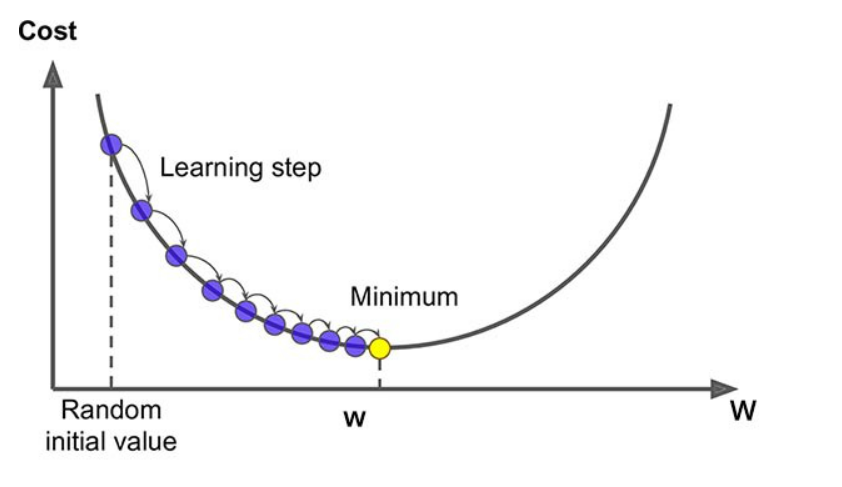
\includegraphics[width=0.7\textwidth]{grad_des}}
\caption{Prikaz delovanja metode gradientnega spusta}
\label{fig:foobar}
\end{figure}


\noindent Težave, ki se pri tem algoritmu pojavijo, so ustrezna izbira vhodnih podatkov. Eden izmed teh je učna stopnja, saj bi radi delali velike korake, kar bi pomenilo manjše število iteracij, vendar se nam lahko zgodi, da s tem zgrešimo našo rešitev in sam algoritem ne vrne prave rešitve, če pa delamo premajhne korake pa je potrebno veliko število iteracij, da pridemo do rešitve. \\
Naslednji izmed vhodnih podatkov je začetna točka $x_0$. Želimo si jo izbrati tako, da je čim bližje optimalni rešitvi, saj bomo zaradi tega potrebovali manj iteracij.


\newpage
\section{Primer uporabe pri linearni regresiji}
Za začetek obravnave algoritem gradientnega spusta sem si pogledala linearno regresijo. Podatki, ki sem jih uporabila so izmišljeni. Opazovala sem predvsem kako se algoritem odziva ob spreminjaju vhodnih podatkov.\\

\noindent Vemo, da gradientni spust doseže optimalno vrednost tako, da na začetku algoritma dela velike korake, ko pa se bliža optimalni vrednosti (minimumu) pa so koraki vedno manjši. To lastnost algoritma lahko potrdi slika 2. Na prvi sliki torej vidimo, da pet dodatnih iteracij zelo vpliva na premico (razlika med pet in deset iteracij), med tem ko na drugi sliki, kjer gledamo razliko med 95 in 100 iteracij, skoraj ni razlike, saj so koraki, ki jih delamo vedno manjši. \\

\begin{figure}[h]
    \centering
    \subfigure{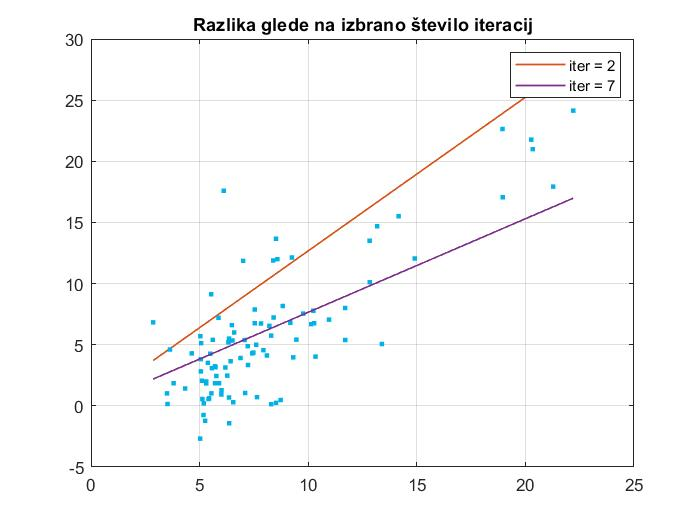
\includegraphics[width=0.45\textwidth]{premica_iter1.jpg}}
    \subfigure{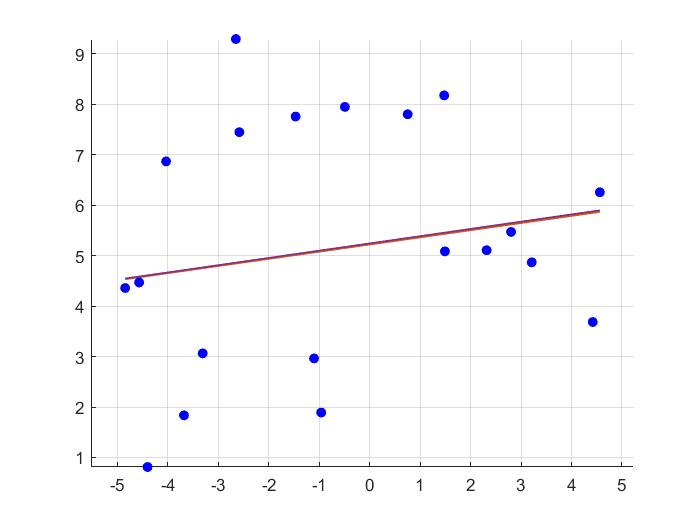
\includegraphics[width=0.45\textwidth]{premica_iter2.jpg}} 
    \caption{Razlike v številu iteracij}
    \label{fig:foobar}
\end{figure}

\noindent V naslednjem poskusu, sem spreminjala začetne pogoje in opazovala koliko iteracij je potrebno, da se premica približa optimalni rešitvi. V primeru a) sem za naklon vzela 20, za konstanto (začetno vrednost) pa -50. Opazimo, da algoritem potrebuje približno 600 iteracij, da se dobro prilega danim podatkom, med tem ko v naslednjem primeru, kjer je naklon enak -20, konstanta pa 50, potrebuje približno 800 iteracij. Sam vzrok takšne razlike je v napačnem predznaku začetnega naklona. V primeru c) sem vzela za začetni naklon in konstanto kar vrednost 1. Opazimo, da sta blizu optimalnemu naklonu in konstanti, zato se že pri desetih iteracijah premica dobro prilega točkam. V tem primeru je torej dobro pogledat podatke in na podlagi tega določit približen naklon in konstanto, saj bo zaradi tega potrebnih manj iteracij.
\begin{figure}[!htb]
    \centering
    \subfigure[naklon = 20, konst = -50]{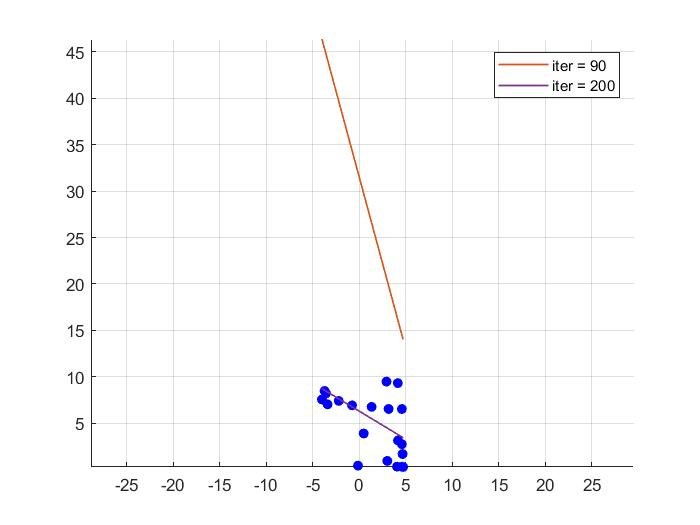
\includegraphics[width=0.45\textwidth]{premica_zp3.jpg}} 
    \subfigure[naklon = -20, konst = 50]{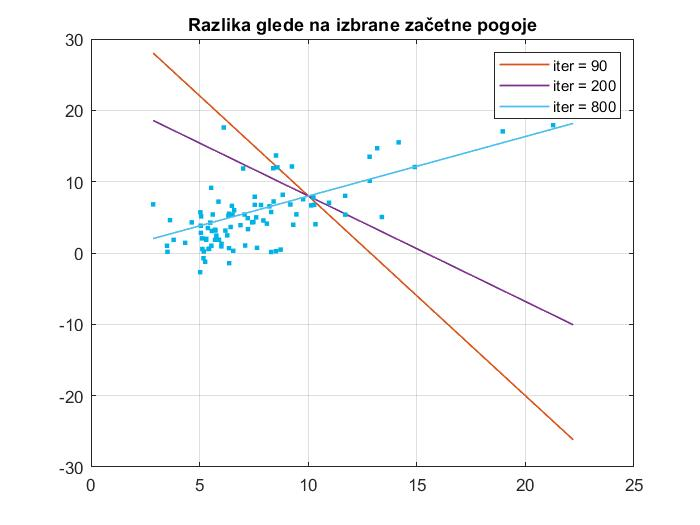
\includegraphics[width=0.45\textwidth]{premica_zp1.jpg}} 
    \subfigure[naklon = 1, konst = 1]{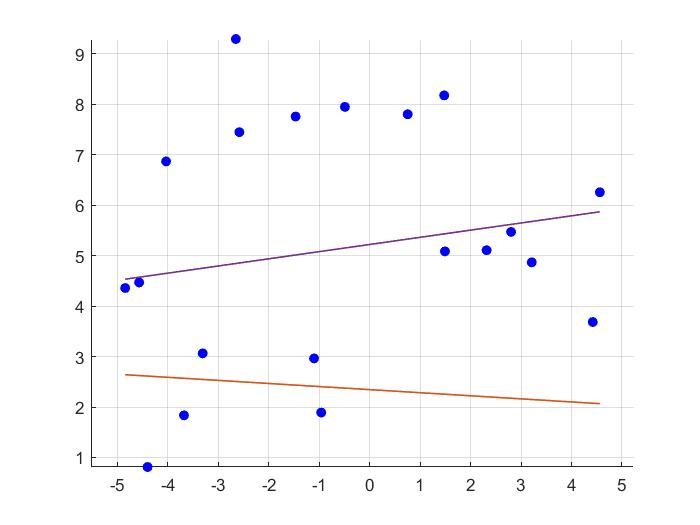
\includegraphics[width=0.45\textwidth]{premica_zp2.jpg}}
    \caption{Razlika pri različnih začetnih pogojih}
    \label{fig:foobar}
\end{figure}

\newpage
\noindent Zanimalo me je tudi, kako se sama premica spreminja pri različno izbranih učnih stopnjah. Naredila sem 100 iteracij za vsako učno stopnjo in ugotovila, da manjša je ta stopnja dlje smo od optimalne rešitve po vseh iteracijah. Kar je seveda smiselno, saj manjša kot je učna stopnja, manjše korake delamo in dlje časa potrebujemo, da se približamo optimalni premici.

\begin{figure}[!htb]
\centering
\subfigure{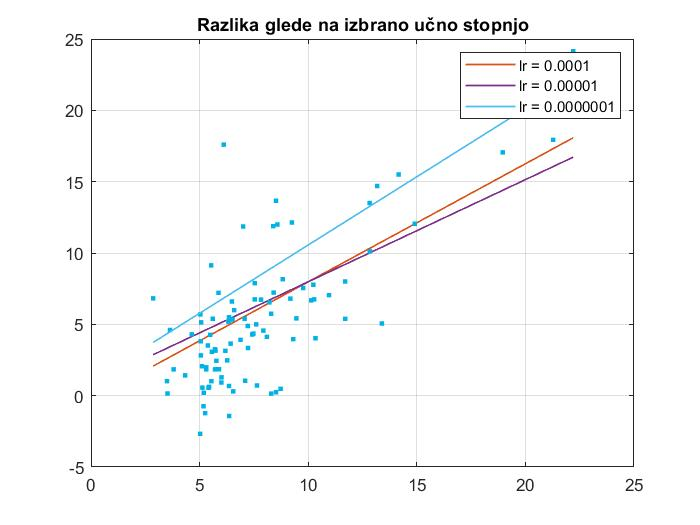
\includegraphics[width=0.5\textwidth]{premica_lr.jpg}} 
\caption{Razlika pri različnih učnih stopnjah}
\label{fig:foobar}
\end{figure}



\newpage
\section{Iskanje minimuma podane funkcije}
V tem poglavju bom predstavila iskanje minimuma funkcije ene in več spremenljivk s pomočjo metode gradientnega spusta. Pogledala sem si enostavne funkcije iz katerih se lepo vidijo prednosti in slabosti te metode.\\
\subsection{Iskanje minimuma funkcije ene spremenljivke}

\noindent Prva težava gradientnega spusta, kot sem že omenila v teoretičnem delu, je izbira učne stopnje. Želimo si izbrati čim večjo, da bo potrebnih čim manj iteracij, ampak se nam lahko zgodi, da bomo minimum preskočili. Pogledala sem si funkcijo $x^2$. Iz spodnjih slik se lepo vidi, kako različne učne stopnje vplivajo na iskanje minimuma in koliko iteracij je potrebnih. Na grafu levo zgoraj, kjer je učna stopnja enaka 0.1, lahko vidimo, da po 42 iteracijah dosežemo neko vrednost dovolj blizu 0. Če za učno stopnjo izberemo 0.3 ali 0.7 potrebujemo 13 iteracij. Opazimo pa tudi da pri učni stopnji 0.7 začnejo vrednosti skakati iz ene strani minimuma na drugo stran, kar je posledica prevelike stopnje. V primeru, ko pa je učna stopnja enaka 0.9 je teh skokov še več in je vrednost dovolj blizu 0 šele pri 52 iteraciji.

\begin{figure}[h]
    \centering
    \subfigure{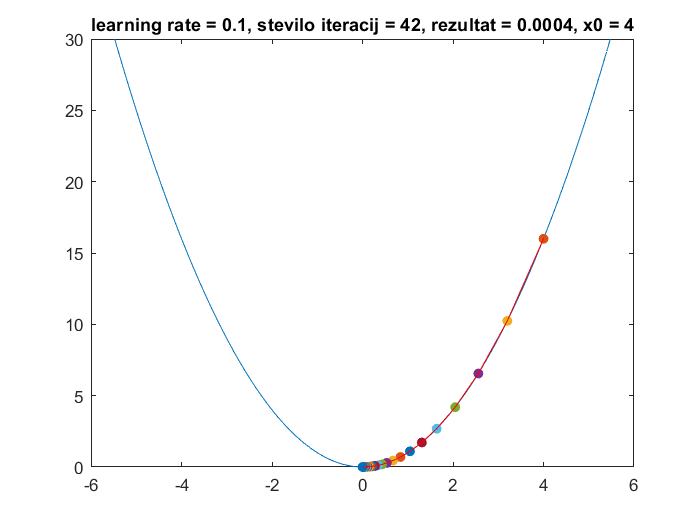
\includegraphics[width=0.45\textwidth]{fun_lepo.png}}
    \subfigure{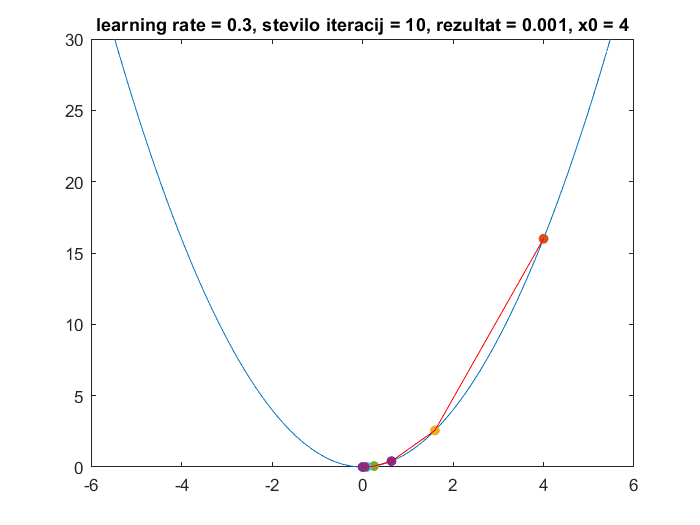
\includegraphics[width=0.45\textwidth]{fun_lepo2.png}} 
    \subfigure{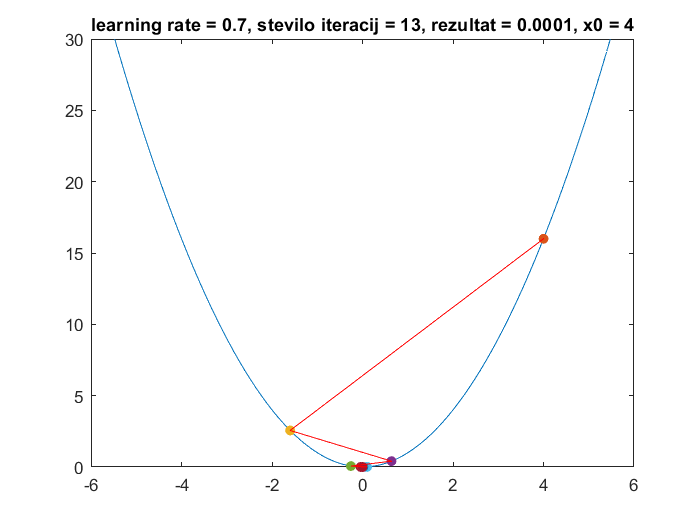
\includegraphics[width=0.45\textwidth]{fun_skace.png}}
    \subfigure{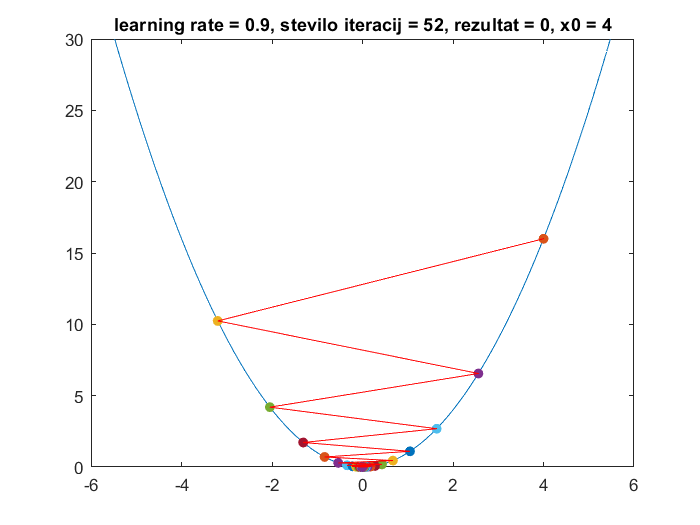
\includegraphics[width=0.45\textwidth]{fun_skace2.png}} 
    \caption{Razlike glede na izbrano učno stopnjo}
    \label{fig:foobar}
\end{figure}

\noindent Za določitev ustrezne učne stopnje si lahko pomagamo z grafom. V primeru funkcije $x^2 $ sta to vrednosti 0.3 in 0.7, ki se dovolj približata ničli v trinajstih iteracijah. Torej za ustrezno učno stopnjo lahko vzamemo vrednosti med 0.3 in 0.7. Tiste, ki pa niso v tem intervalu bodo potrebovale več iteracij, da bodo dovolj blizu minimuma.  \\


\begin{figure}[!htb]
    \centering
    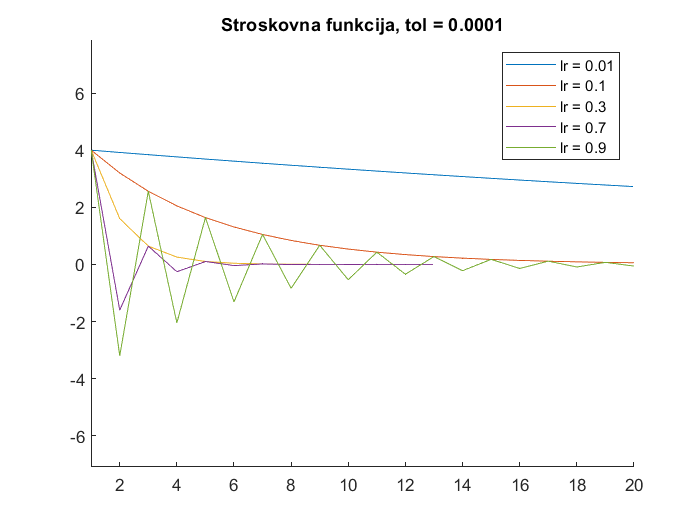
\includegraphics[scale=0.5]{str_fun}   
    \caption{Izravnana funkcija}
    \label{fig:foobar}
\end{figure}


\noindent Naslednja stvar, ki sem jo opazila je, da sam algoritem ni primeren za funkcije, ki so nekaj časa skoraj konstantna oz. je naklon tangente skoraj ničelni. Pri takih funkcijah sam algoritem potrebuje veliko več iteracij, da pride do minimuma, saj dela majhne korake. Na spodnjem grafu funkcije $\frac{x^2}{1000}$ vidimo, da je kljub dobro izbrani učni stopnji končna vrednost približka po 1000 iteracijah za minimum enaka 0.8066, kar je še vedno daleč stan od samega minimuma.


\begin{figure}[h]
    \centering
    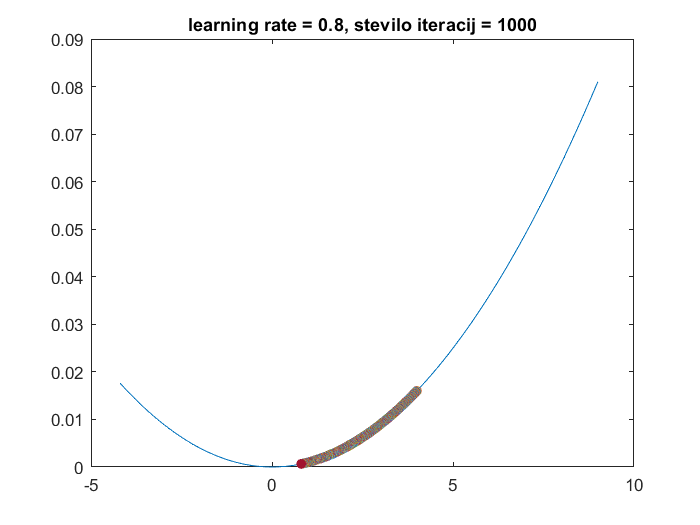
\includegraphics[scale=0.5]{izravnana_fun}   
    \caption{Izravnana funkcija}
    \label{fig:foobar}
\end{figure}

\newpage
\noindent Zanimiv primer za obravnavo je naslednja funkcija: $x^4-2x^3+2$. Težave algoritmu povzroči sedlo, torej funkcija ni strogo konveksna. To je lep primer iz katerega so vidne težave algoritma. Vrednost, ki nam jo vrne metoda gradientnega spusta je zelo odvisna od izbire začetne točke in učne stopnje. \\

\noindent V primeru, ko za začetni približek vzamemo $x_0 = 2$, lahko opazimo, da nam pri učni stopnji 0.1 algoritem vrne globalni minimum, pri učni stopnji 0.3 pa lokalni minimum, saj delamo velike korake in s tem preskočimo globalni minimum. Prav tako je zanimiva situacija v primeru, ko za $x_0$ vzamemo vrednost -0.5. V primeru učne stopnje 0.1 algoritem vrne lokalni minimum, v primeru 0.3 globalni minimum, v primeru 0.4 pa obišče tako globalni kot lokalni minimum in potem obstoji v lokalnemu, ne glede na to koliko iteracij naredimo. Iz tega primera se lahko torej naučimo, da pri tem algoritmu nikoli ne vemo ali nam vrne globalni ali lokalni minimum.

\begin{figure}[!htb]
    \centering
    \subfigure{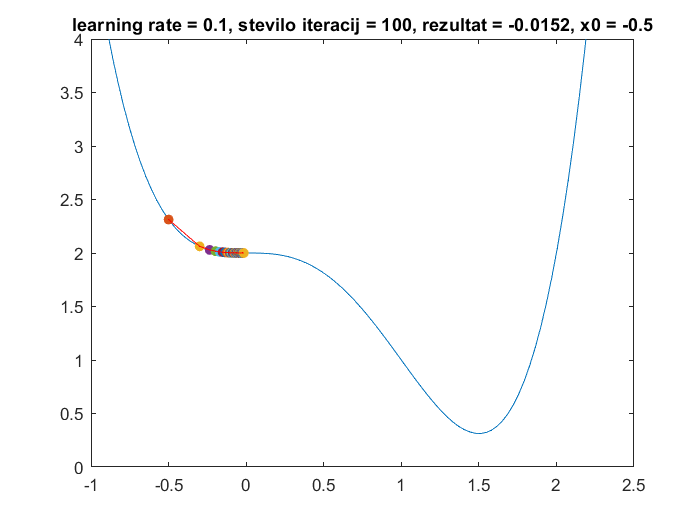
\includegraphics[width=0.45\textwidth]{sedlo1.png}}
    \subfigure{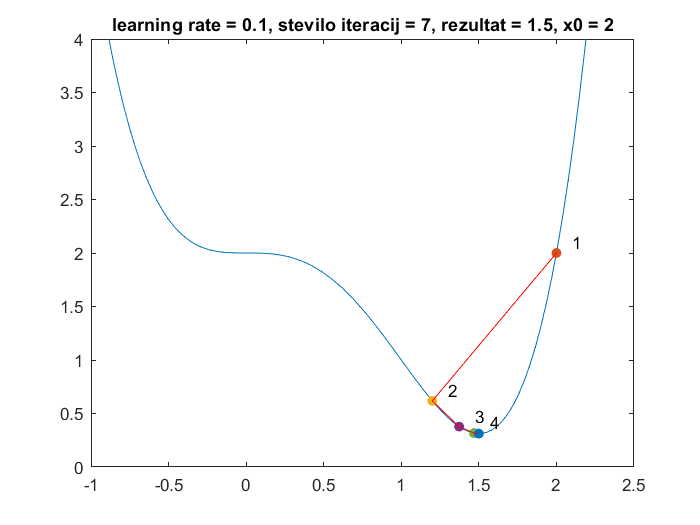
\includegraphics[width=0.45\textwidth]{sedlo2.png}} 
\end{figure}


\begin{figure}[!htb]
    \centering
    \subfigure{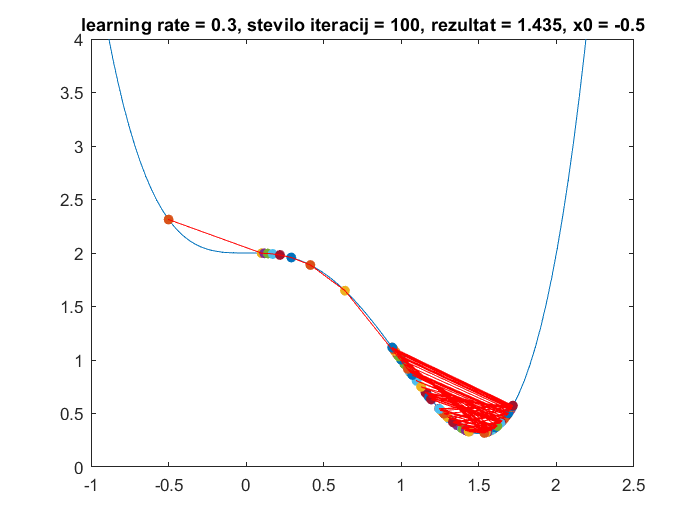
\includegraphics[width=0.45\textwidth]{sedlo3.png}}
    \subfigure{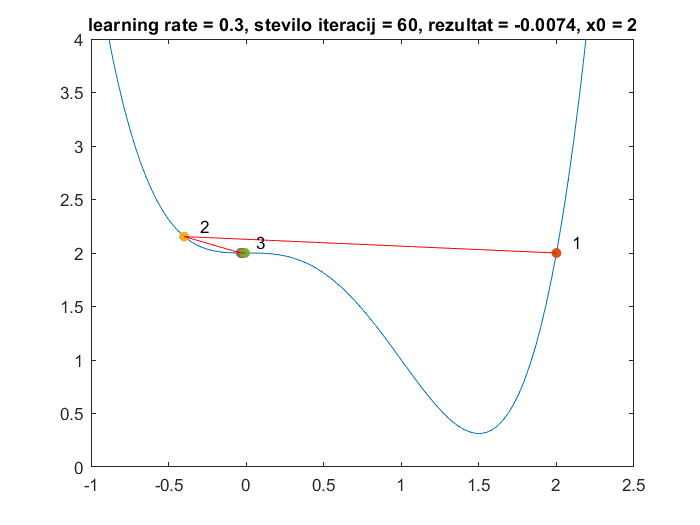
\includegraphics[width=0.45\textwidth]{sedlo4.png}} 
    \subfigure{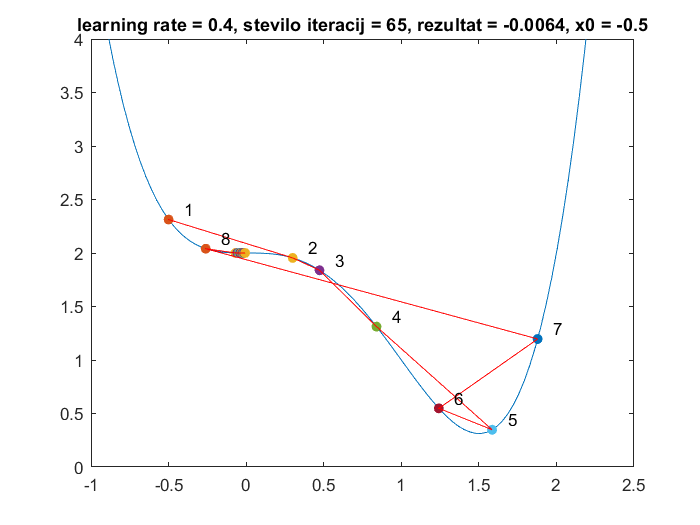
\includegraphics[width=0.45\textwidth]{sedlo5.png}} 
    \caption{Razlike glede na izbrano učno stopnjo in začetni približek}
    \label{fig:foobar}
\end{figure}

\noindent Tudi če pogledamo graf za lažje določanje ustrezne učne stopnje nam le ta vrne, da pri začetni točki $x_0 = 2$ je najbolj ustrezna učna stopnja 0.4. Ampak iz zgornjih grafov vidimo, da nam le ta ne vrne globalnega minimuma, ampak lokalni minimum.
\begin{figure}[!htb]
    \centering
    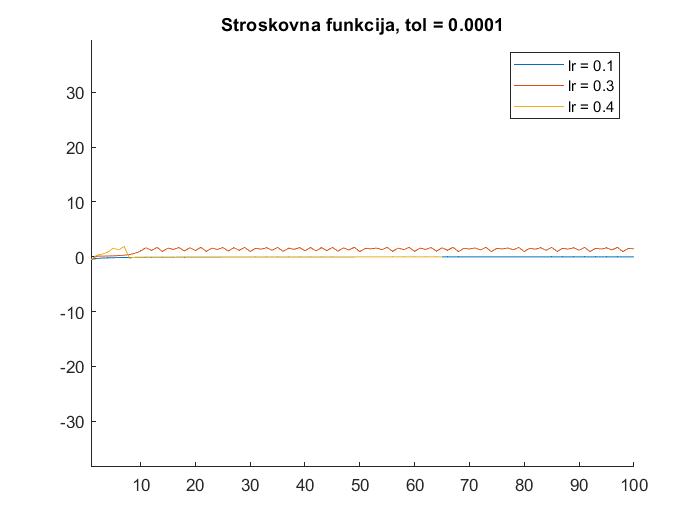
\includegraphics[scale=0.4]{str_fun2}   
    \caption{Izravnana funkcija}
    \label{fig:foobar}
\end{figure}

\newpage
\subsection{Iskanje minimuma funkcije več spremenljivk}
Podobno kot pri iskanju minimuma funkcije ene spremenljivke si lahko za začetek pogledamo funkcijo $x^2+y^2$. V primeru, ko je učna stopnja enaka 0.8 lahko opazimo, da tako x koordinate kot y koordinate skačejo iz pozitivnih v negativna števila in dosežejo minimum v 19 iteracijah, med tem ko pri učni stopnji 0.1 so vrednosti obeh koordinat pozitivne in lepo padajo k minimumu. V tem primeru pa je potrebnih 31 iteracij.\\

\begin{figure}[h]
    \centering
    \subfigure{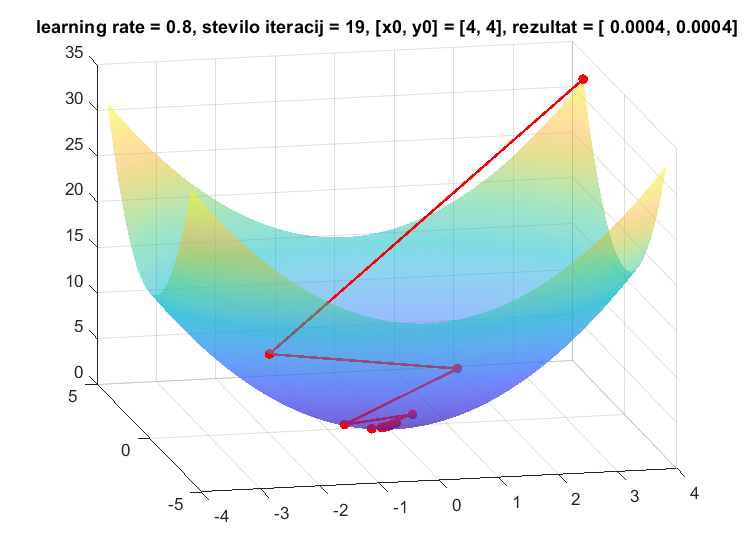
\includegraphics[width=0.45\textwidth]{skacevec.png}}
    \subfigure{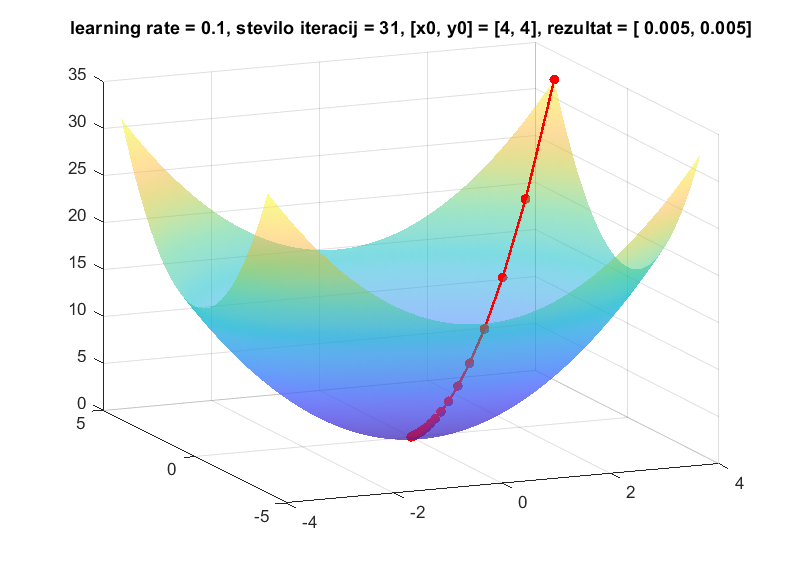
\includegraphics[width=0.45\textwidth]{lepovec.png}} 
    \caption{Razlike glede na izbran learning rate}
    \label{fig:foobar}
\end{figure}


\noindent Če si pogledamo funkcijo, ki ima sedla in več lokalnih minimumov opazimo podobne stvari, kot v primeru funkcij ene spremenljivke. Samo iskanje minimuma je zelo odvisno od izbire začetnega približka in učne stopnje. Na spodnjih grafih opazimo, da pri različnih učnih stopnjah metoda najde različne minimume. Prav tako je razlika v konvergenci, nekje lepo pada proti minimumu, nekje pa skače iz ene strani minimuma na drugo stran.

\begin{figure}[h]
    \centering
    \subfigure{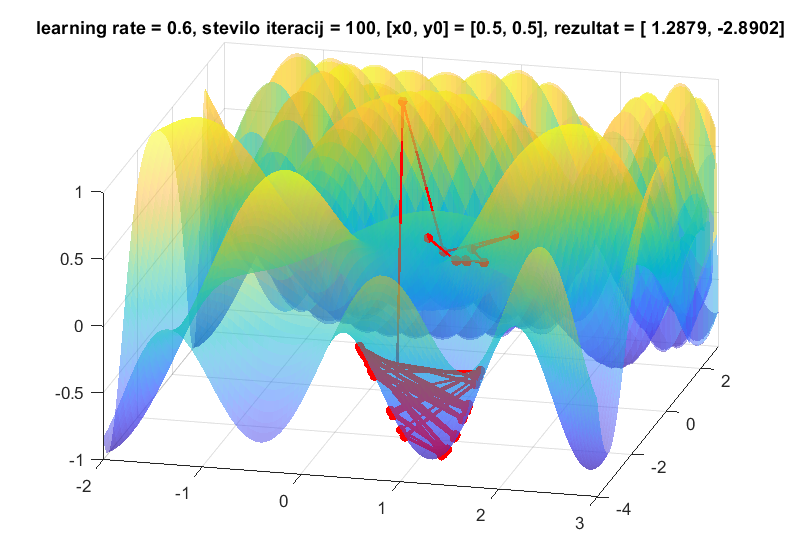
\includegraphics[width=0.45\textwidth]{sedlo1vec.png}}
    \subfigure{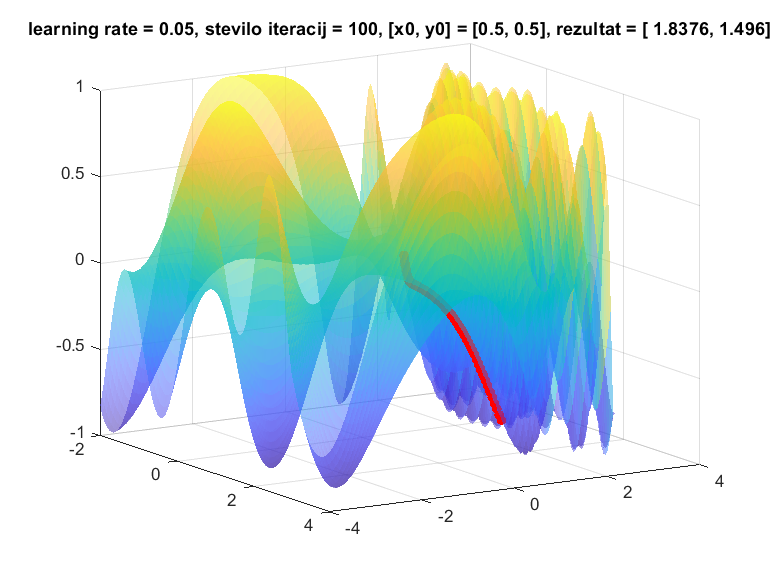
\includegraphics[width=0.45\textwidth]{sedlo2vec.png}} 
    \caption{Razlike glede na izbran learning rate}
    \label{fig:foobar}
\end{figure}

\newpage
\section{Zaključek}
Iz grafov in izračunov sem ugotovila, da je sam algoritem najbolj odvisen od učne stopnje in začetnega približka. Od tega je odvisno število iteracij. Sama učna stopnja vpliva tudi na konvergenco/divergenco algoritma ter na hitrost konvergence. Algoritem, kot sem že omenila, je primeren samo za konveksne in diferenciabilne funkcije, saj drgače konvergenca ni zagotovljena, kot smo lahko tudi videli v četrtem poglavju. \\
To projektno nalogo bi bilo smiselno tudi razširit, saj poznamo različne metode in variacije gradientnega spusta, ki so uporabne. Ena izmed njih, ki sem jo velikokrat zasledila, je gradientni spust z momentom, ki reši težavo, ko se vrednost ujame v lokalni minimum. Enačba je v tem primeru sledeča
\[ x_{t+1} =\lambda x_t - \eta {\nabla f(x)}.\]
Smiselno bi bilo tudi pogledati še za različne funkcije, tudi v višjih dimenzijah. Lahko bi tudi trigonometričnim funkcijami poiskali polinome, ki se jim najbolje prilegajo. Mislim, da je možnosti za razširitev zelo veliko.



\pagebreak
\begin{thebibliography}{9}
\bibitem{texbook}
Nisheeth K. Vishnoi (2020) \emph{Algorithms for Convex Optimization}. Pridobljeno 24. 4. 2022 iz \url{https://convex-optimization.github.io/}.

\bibitem{lamport94}
Robert Kwiatkowski (2021) \emph{Gradient Descent Algorithm — a deep dive}. Pridobljeno 30. 4. 2022 iz \url{https://towardsdatascience.com/gradient-descent-algorithm-a-deep-dive-cf04e8115f21}.

\end{thebibliography}
\end{document}